\section{Metodologia}\label{sec:metodologia}

Para responder à pergunta do estudo, eram necessárias duas medidas para cada classe diagnóstica: o desempenho do modelo e a qualidade das explicações das suas predições. O estudo foi, por isso, experimental e descritivo, com a classe como unidade de comparação (Fig.~\ref{fig:pipeline}). Um classificador multirrótulo foi treinado, e o seu desempenho em cada classe foi medido pelo F1 no conjunto de teste. As predições corretas desse conjunto foram explicadas pelo GradientSHAP, cada explicação foi resumida em regiões do batimento, e a qualidade das explicações foi medida por sete métricas de quatro categorias, para que a pergunta fosse respondida para várias propriedades, e não para uma só. Por fim, a ordem das classes em cada métrica foi comparada com a ordem pelo F1. Todo o código e os resultados estão em um repositório público\footnote{\url{https://github.com/Arthur-so/shap-ecg-arrhythmia}}.

\begin{figure*}[!t]\centering
\begin{tikzpicture}[node distance=5mm and 7mm]
\node[dado] (d) {CPSC2018\\6\,877 ECGs\\12 derivações};
\node[proc, right=of d] (p) {Pré-processamento\\(Seção~\ref{sec:dados})};
\node[proc, right=of p] (m) {Treino da\\ResNet34-1D\\(Seção~\ref{sec:modelo})};
\node[saida, right=of m] (f) {F1 por classe\\no teste};
\node[proc, below=8mm of m] (g) {GradientSHAP\\622 mapas\\(Seção~\ref{sec:gshap})};
\node[proc, left=of g] (r) {36 regiões\\do batimento\\(Seção~\ref{sec:regioes})};
\node[proc, left=of r] (mt) {7 métricas + piso\\(Seções~\ref{sec:piso}\\e~\ref{sec:metricas})};
\node[saida, right=of g] (c) {Comparação\\descritiva\\(Seção~\ref{sec:analise})};
\draw[seta] (d) -- (p); \draw[seta] (p) -- (m); \draw[seta] (m) -- (f);
\draw[seta] (m) -- (g); \draw[seta] (g) -- (r); \draw[seta] (r) -- (mt);
\draw[seta] (f) -- (c);
\draw[seta] (mt.south) -- ++(0,-4mm) -| (c.south);
\end{tikzpicture}

\caption{Etapas do estudo. O desempenho do modelo (F1 por classe, em cima) e a qualidade das explicações (métricas por classe, embaixo) foram obtidos para as mesmas classes e comparados ao final.}\label{fig:pipeline}
\end{figure*}

\subsection{Base de dados e pré-processamento}\label{sec:dados}
Foi usada a base do \textit{China Physiological Signal Challenge} 2018 (CPSC2018)~\cite{liu2018}, na distribuição do desafio PhysioNet/CinC 2020~\cite{perezalday2020}: 6\,877 ECGs de 12 derivações amostrados a 500~Hz, com duração de 6 a 60~s~\cite{zhang2021}. Os rótulos foram lidos dos códigos SNOMED CT dos cabeçalhos e mapeados para nove classes: ritmo sinusal normal (SNR), fibrilação atrial (AF), bloqueio atrioventricular de 1.º grau (IAVB), bloqueio de ramo esquerdo (BRE), bloqueio de ramo direito (BRD), contração atrial prematura (CAP), contração ventricular prematura (CVP), depressão do segmento ST (STD) e elevação do segmento ST (STE). Como 476 registros (6,9\%) tinham mais de um diagnóstico, o problema foi tratado como multirrótulo. A Tabela~\ref{tab:classes} mostra o número de registros por classe.

\begin{table}[!t]\centering
\caption{Registros por classe em cada partição. Um registro pode ter mais de um rótulo.}\label{tab:classes}
\setlength{\tabcolsep}{4pt}
\begin{tabular}{lrrrr}
\toprule
\textbf{Classe} & \textbf{Treino} & \textbf{Validação} & \textbf{Teste} & \textbf{Total} \\
\midrule
SNR  & 642 & 184 & 92 & 918 \\
AF   & 858 & 242 & 121 & 1\,221 \\
IAVB & 503 & 144 & 75 & 722 \\
BRE  & 165 & 47 & 24 & 236 \\
BRD  & 1\,304 & 371 & 182 & 1\,857 \\
CAP  & 431 & 122 & 63 & 616 \\
CVP  & 491 & 140 & 69 & 700 \\
STD  & 609 & 172 & 88 & 869 \\
STE  & 154 & 44 & 22 & 220 \\
\midrule
Registros & 4\,812 & 1\,378 & 687 & 6\,877 \\
\bottomrule
\end{tabular}
\end{table}

Como a rede exige entradas de tamanho fixo, cada registro foi truncado ou completado com zeros até 15\,000 amostras (30~s), o mesmo comprimento usado por Zhang et al.~\cite{zhang2021}. Diferentemente da referência, que mantém os últimos 30~s dos registros longos e não normaliza o sinal~\cite{zhang2021}, foram mantidos os primeiros 30~s, e cada derivação foi normalizada por \textit{z-score}; por isso, as amplitudes estão em unidades de desvio padrão. Os registros foram divididos em treino, validação e teste (70\%, 20\% e 10\%), de forma estratificada por classe e com semente fixa. O comprimento real de cada registro foi guardado para excluir o preenchimento de todas as análises por região, já que a duração mediana dos registros era de 12~s.

\subsection{Modelo e treino}\label{sec:modelo}
Foi usada a ResNet34 unidimensional de Zhang et al.~\cite{zhang2021}, por ser a arquitetura de referência na mesma base, adaptada das redes residuais de He et al.~\cite{he2016}, em que cada bloco aprende um resíduo em relação à sua entrada, somada à saída por uma conexão de atalho (Fig.~\ref{fig:resnet}). As 12 derivações entram na rede como canais; dezesseis blocos residuais em quatro estágios reduzem o sinal a 512 canais × 469 instantes; a média e o máximo ao longo do tempo formam um vetor de 1\,024 valores; e uma camada linear produz um logit $z_c$ por classe. A probabilidade de cada classe foi obtida por uma sigmoide independente, $p_c = 1/(1+e^{-z_c})$, porque um ECG pode ter mais de um diagnóstico, e a classe foi considerada predita quando $p_c$ atingiu o limiar $t_c$ da classe.

\begin{figure*}[!t]\centering
\begin{tikzpicture}[node distance=3mm and 3.2mm, every node/.style={font=\scriptsize}]
\node[dado, minimum height=11mm] (in) {ECG\\12 × 15\,000};
\node[proc, right=of in, minimum height=11mm] (st) {Conv 15, /2\\BN, ReLU\\MaxPool /2};
\node[proc, right=of st, minimum height=11mm, fill=orange!15] (s1) {Estágio 1\\3 blocos};
\node[proc, right=of s1, minimum height=11mm, fill=orange!22] (s2) {Estágio 2\\4 blocos, /2};
\node[proc, right=of s2, minimum height=11mm, fill=orange!30] (s3) {Estágio 3\\6 blocos, /2};
\node[proc, right=of s3, minimum height=11mm, fill=orange!38] (s4) {Estágio 4\\3 blocos, /2};
\foreach \n/\t in {in/{12 × 15\,000}, st/{64 × 3\,750}, s1/{64 × 3\,750}, s2/{128 × 1\,875}, s3/{256 × 938}, s4/{512 × 469}}
  \node[nota, below=0.5mm of \n] {\t};
\node[proc, below=11mm of s4, minimum height=11mm] (pool) {Média e máximo\\no tempo};
\node[proc, below=11mm of s3, minimum height=11mm] (fc) {Linear\\1\,024 → 9};
\node[proc, below=11mm of s2, minimum height=11mm] (sig) {Sigmoide\\por classe};
\node[proc, below=11mm of s1, minimum height=11mm] (lim) {$p_c \ge t_c$\,?};
\node[saida, below=11mm of st, minimum height=11mm] (out) {Classes\\preditas};
\node[nota, below=0.5mm of pool] {1\,024};
\node[nota, below=0.5mm of fc] {9 logits\\$z_c$};
\node[nota, below=0.5mm of sig] {9 probabilidades\\$p_c$};
\node[nota, below=0.5mm of lim] {limiar $t_c$\\por classe};
\draw[seta] (in)--(st); \draw[seta] (st)--(s1); \draw[seta] (s1)--(s2); \draw[seta] (s2)--(s3); \draw[seta] (s3)--(s4);
\draw[seta] (s4)--(pool); \draw[seta] (pool)--(fc); \draw[seta] (fc)--(sig); \draw[seta] (sig)--(lim); \draw[seta] (lim)--(out);
% bloco residual
\begin{scope}[shift={(1.2,-4.75)}, node distance=2.6mm]
\node[font=\scriptsize\bfseries, anchor=east] (tit) at (-0.85,0) {Bloco residual:};
\node[caixa, font=\scriptsize] (x) {entrada};
\node[caixa, right=of x, font=\scriptsize] (c1) {Conv 7};
\node[caixa, right=of c1, font=\scriptsize] (b1) {BN, ReLU};
\node[caixa, right=of b1, font=\scriptsize] (dp) {\textit{Dropout} 0,2};
\node[caixa, right=of dp, font=\scriptsize] (c2) {Conv 7};
\node[caixa, right=of c2, font=\scriptsize] (b2) {BN};
\node[circle, draw, right=of b2, inner sep=1pt, font=\scriptsize] (sum) {$+$};
\node[caixa, right=of sum, font=\scriptsize] (rl) {ReLU};
\draw[seta] (x)--(c1); \draw[seta] (c1)--(b1); \draw[seta] (b1)--(dp); \draw[seta] (dp)--(c2); \draw[seta] (c2)--(b2); \draw[seta] (b2)--(sum); \draw[seta] (sum)--(rl);
\draw[seta] (x.south) -- ++(0,-4mm) -| (sum.south);
\node[nota, below=4.5mm of dp] {atalho: a entrada é somada à saída (com Conv 1 × 1, /2, quando o comprimento muda)};
\end{scope}
\end{tikzpicture}

\caption{Arquitetura da ResNet34-1D: o ECG atravessa quatro estágios de blocos residuais, é resumido no tempo e produz um logit e uma probabilidade por classe. Abaixo de cada etapa, a dimensão da saída (canais × instantes); embaixo, um bloco residual, em que a entrada é somada à saída. Elaborada com base em~\cite{zhang2021}.}\label{fig:resnet}
\end{figure*}

O treino usou entropia cruzada binária sem ponderação, otimizador Adam com taxa de aprendizado $10^{-4}$, lotes de 32 ECGs, \textit{dropout} de 0,2 nos blocos e aumento de dados por escala e deslocamento da linha de base de cada derivação, como na referência~\cite{zhang2021}. O treino foi limitado a 60 épocas, com parada antecipada após 10 épocas sem melhora do F1-macro na validação, e foi mantido o modelo da melhor época; a referência usa no máximo 30 épocas~\cite{zhang2021}. Para verificar se o desbalanceamento entre as classes exigia uma perda ponderada, foi treinado também um modelo com a entropia cruzada ponderada pela frequência de cada classe, nas mesmas condições.

Como o limiar que maximiza o F1 em geral não é 0,5 e depende da classe~\cite{lipton2014}, o limiar de cada classe foi escolhido na validação, testando valores de 0,00 a 1,00 em passos de 0,01 e escolhendo o de maior F1, e depois aplicado sem mudança ao teste, como em~\cite{zhang2021}. O desempenho foi medido pelo F1 de cada classe no teste, e o F1-macro, a média das nove classes, foi usado como resumo.

\subsection{Explicações GradientSHAP}\label{sec:gshap}
Para cada ECG $x$ e classe $c$, o GradientSHAP, na implementação do Captum~\cite{kokhlikyan2020}, produziu um mapa $\phi$ com a mesma dimensão do ECG (12 × 15\,000), que atribui a cada ponto uma parcela do logit $z_c$. O método aproxima os valores SHAP~\cite{lundberg2017} por gradientes calculados ao longo do caminho entre referências e a entrada, como nos gradientes integrados~\cite{sundararajan2017}. Em cada um de $M = 200$ sorteios, foram sorteados uma referência $r_m$ e um ruído gaussiano somado ao ECG, $\tilde{x}_m = x + \varepsilon_m$; foi sorteado um ponto $x'_m = r_m + \alpha_m(\tilde{x}_m - r_m)$ do caminho entre os dois, com $\alpha_m \in [0,1]$; e o gradiente nesse ponto foi multiplicado pela diferença entre o ECG e a referência (Fig.~\ref{fig:gshap}). O mapa é a média dos sorteios:
\begin{equation}
\phi(x) = \frac{1}{M}\sum_{m=1}^{M} \nabla z_c(x'_m) \odot (\tilde{x}_m - r_m).
\label{eq:gshap}
\end{equation}

\begin{figure*}[!t]\centering
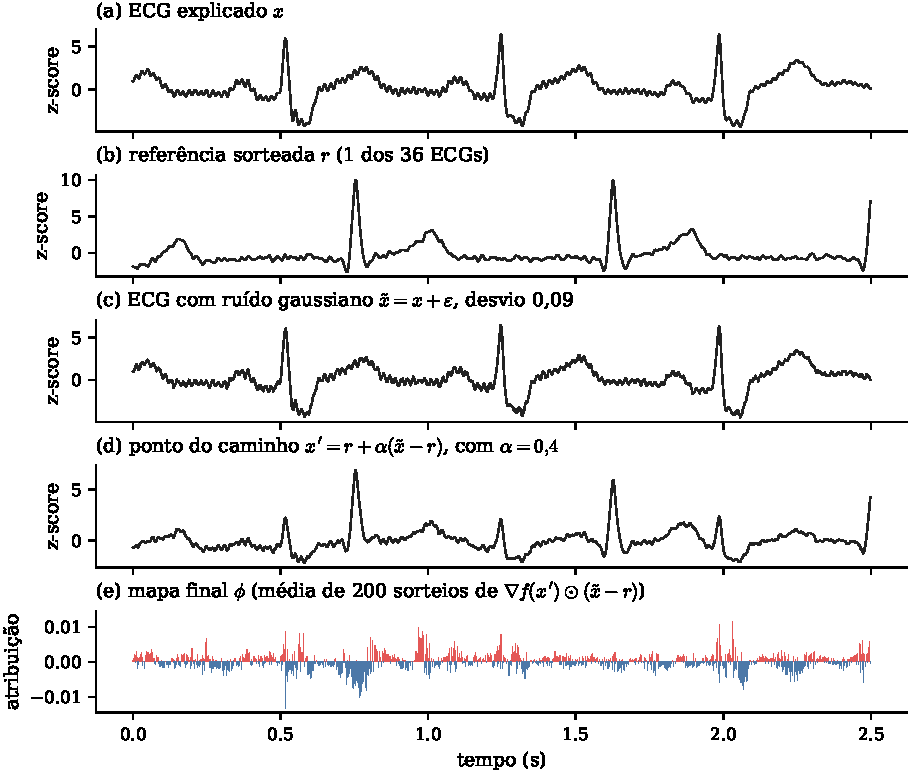
\includegraphics[width=0.6\textwidth]{figs/gshap.pdf}
\caption{Construção de um mapa GradientSHAP com sinais reais (derivação II de um ECG de BRD). Os painéis (a) a (d) mostram um sorteio: (a) ECG; (b) uma das 36 referências; (c) ECG com ruído; (d) ponto do caminho em que o gradiente é calculado. O painel (e) mostra o mapa final, média de 200 sorteios, com a atribuição positiva em vermelho e a negativa em azul; os maiores valores ficam nos complexos QRS.}\label{fig:gshap}
\end{figure*}

As referências foram 36 ECGs do treino com um único rótulo, quatro de cada classe, sorteados com semente fixa. Usar uma distribuição de ECGs reais como referência segue Turbé et al.~\cite{turbe2023}, que usaram 50 ECGs na mesma base; o balanceamento evita que a referência represente sobretudo as classes mais frequentes. O ruído suaviza oscilações locais do gradiente, como no SmoothGrad~\cite{smilkov2017}; o desvio usado, 0,09, é o do exemplo de uso do Captum e não foi ajustado. O número de sorteios foi aumentado de 50 para 200 depois que a variação entre mapas do mesmo ECG com sementes diferentes (Seção~\ref{sec:piso}) se mostrou alta com 50; com 200, essa variação caiu à metade. Foram explicadas apenas as predições corretas do teste: para cada registro, um mapa para cada classe presente e predita, num total de 622 mapas.

\subsection{Regiões do batimento}\label{sec:regioes}
Cada mapa tinha 180\,000 valores. As métricas, porém, foram calculadas sobre 36 regiões, e não sobre pontos, por três motivos. Primeiro, retirar pontos isolados quase não altera a saída do modelo e incluía o preenchimento, que ocupa a maior parte do mapa na maioria dos ECGs; perturbar trechos contíguos introduz menos ruído de alta frequência no sinal~\cite{cui2023}; agrupar pontos consecutivos melhorou as métricas de perturbação em séries temporais multivariadas~\cite{serramazza2024}; e perturbações mínimas de pontos podem mudar bruscamente a predição por deslocamento de distribuição, o que levou à recomendação de perturbar regiões de tamanho fixo~\cite{simic2025}. Segundo, regiões como o QRS de V1 têm significado clínico. Terceiro, somar pontos reduz o ruído do mapa: numa verificação preliminar, a distância normalizada entre dois mapas do mesmo ECG com sementes diferentes (Seção~\ref{sec:piso}) foi de 0,53 nos 180\,000 pontos e de 0,18 nas 36 regiões. A agregação entre batimentos também reduz o ruído dos métodos de gradiente em ECG~\cite{wagner2024}.

Os picos R foram detectados na derivação II com o NeuroKit2~\cite{makowski2021}, e cada batimento completo, entre dois picos R, foi dividido em três segmentos (Fig.~\ref{fig:regioes}): QRS, de $R - 80$~ms a $R + 100$~ms; ST-T, de $R + 100$~ms a $R + 0{,}45 \cdot RR$; e pré-QRS, de $R + 0{,}45 \cdot RR$ até 80~ms antes do pico R seguinte, que contém a onda P e o intervalo PR. Janelas fixas em torno do pico R também foram usadas por Wagner et al.~\cite{wagner2024} (300~ms antes e 500~ms depois do pico R) e por Turbé et al.~\cite{turbe2023} (0,35~s antes e 0,55~s depois). A delineação de cada onda pelo NeuroKit2 foi testada e descartada, porque indicava ondas P em ECGs de fibrilação atrial e não reconhecia o QRS alargado dos bloqueios de ramo.

\begin{figure*}[!t]\centering
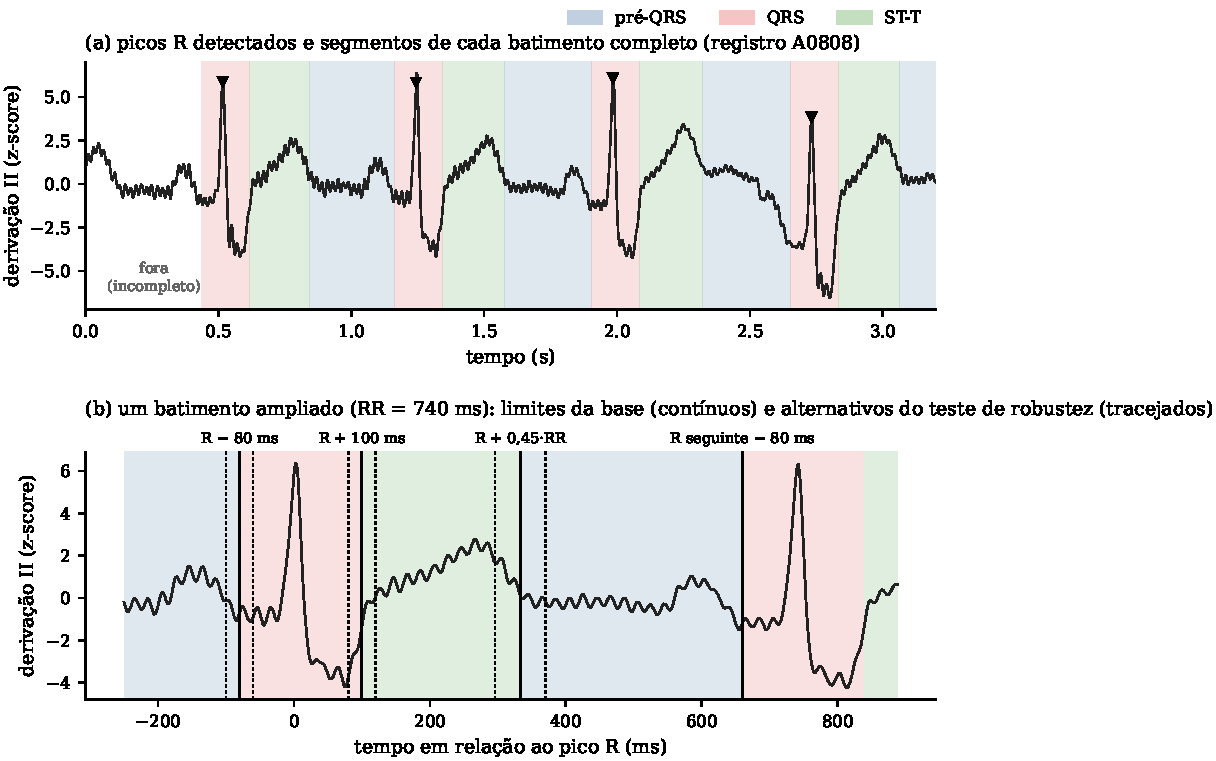
\includegraphics[width=0.72\textwidth]{figs/regioes.pdf}
\caption{Segmentos do batimento definidos a partir dos picos R, num ECG de BRD (derivação II). (a) Picos R detectados e os três segmentos de cada batimento completo; o trecho antes do primeiro pico R fica de fora. (b) Um batimento ampliado, com os limites usados (linhas contínuas) e os limites alternativos do teste de robustez (tracejadas).}\label{fig:regioes}
\end{figure*}

A janela de 180~ms cobre o QRS normal e o QRS alargado dos bloqueios de ramo, definidos por duração de 120~ms ou mais~\cite{hicks2021}; ela é maior depois do pico R porque, nesses bloqueios, o atraso de condução alonga sobretudo a parte final do QRS. O fim do ST-T foi definido como fração do intervalo RR, porque o QT encurta quando a frequência aumenta. Pela fórmula de Bazett, $QT_c = QT/\sqrt{RR}$, a correção mais usada na clínica~\cite{vandenberk2016}, um $QT_c$ de 0,44~s ocupa 0,44 do RR a 60~bpm e 0,50 a 77~bpm, a frequência mediana dos ECGs explicados. Como essa fórmula sobrecorrige o QT em frequências altas~\cite{vandenberk2016}, o fim da onda T pode cair no pré-QRS nos ECGs mais rápidos (17\% dos explicados estavam acima de 100~bpm). Como esses limites são aproximações, foram variados num teste de robustez: janela do QRS de 140, 180 ou 220~ms e fim do ST-T em 0,40, 0,45 ou 0,50 do RR, em 9 combinações, recalculando as métricas que dependem só do mapa e das regiões (\CS\ e \CX). As demais exigiriam passar pelo modelo os ECGs modificados em cada combinação e não foram recalculadas.

A importância de uma região foi definida como a soma do mapa nos pontos daquele segmento, em todos os batimentos completos, numa derivação (Fig.~\ref{fig:agregacao}):
\begin{equation}
A_{d,s} = \sum_{b} \sum_{t \in s(b)} \phi_{d,t},
\label{eq:regiao}
\end{equation}
em que $d$ é a derivação, $s$ o segmento e $b$ percorre os batimentos completos. Cada mapa foi, assim, resumido num vetor de 36 valores. A soma, e não a média usada por Wagner et al.~\cite{wagner2024}, foi escolhida porque é a quantidade que as métricas de retirada comparam com a queda da saída, e porque Zhang et al.\ também resumem os valores SHAP pela soma ao longo do tempo~\cite{zhang2021}.

\begin{figure*}[!t]\centering
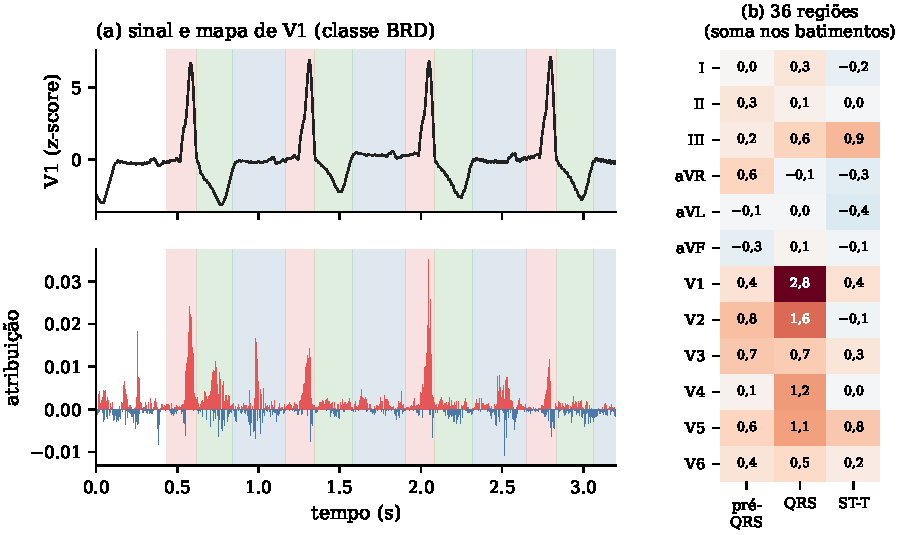
\includegraphics[width=0.74\textwidth]{figs/agregacao.pdf}
\caption{Resumo de um mapa nas 36 regiões (ECG de BRD): o mapa, que oscila ponto a ponto, concentra-se nos QRS, e no vetor das regiões o maior valor é o QRS de V1. (a) Sinal e mapa da derivação V1 nos primeiros 3,2~s, com os segmentos sombreados. (b) Vetor das 36 regiões do ECG inteiro; cada valor é a soma do mapa naquela derivação e segmento, em todos os batimentos completos.}\label{fig:agregacao}
\end{figure*}

\subsection{Variação própria do método: o piso}\label{sec:piso}
Como o GradientSHAP sorteia referências, ruído e pontos do caminho, dois mapas do mesmo ECG com sementes diferentes não são iguais. O \emph{piso} de um mapa foi definido como a distância euclidiana entre esses dois mapas, cada um resumido nas 36 regiões e normalizado para norma 1; ele vai de 0 (mapas iguais) a 2 (opostos). As três métricas que comparam mapas (\MS\ e \AS, \RL\ e \EM) foram calculadas com a mesma semente do mapa original, de modo que só muda o ECG, a classe ou o modelo, e a distância obtida foi lida em relação ao piso (Fig.~\ref{fig:piso}). Sem normalização, métodos cujos escores têm escala menor podem parecer menos sensíveis só por causa da escala~\cite{fouladgar2022}. 

\begin{figure*}[!t]\centering
\begin{tikzpicture}[node distance=4mm and 5mm, every node/.style={font=\scriptsize}]
\node[dado] (x) {ECG $x$,\\classe $c$};
\node[proc, right=10mm of x, yshift=6mm] (g1) {GradientSHAP\\semente $s_1$};
\node[proc, right=10mm of x, yshift=-6mm] (g2) {GradientSHAP\\semente $s_2$};
\node[proc, right=of g1] (v1) {36 regiões,\\norma 1};
\node[proc, right=of g2] (v2) {36 regiões,\\norma 1};
\node[saida, right=12mm of v1, yshift=-6mm] (p) {\textbf{piso}\\$\lVert \hat{a}_1 - \hat{a}_2 \rVert_2$\\(média 0,18)};
\draw[seta] (x.east) -- (g1.west); \draw[seta] (x.east) -- (g2.west);
\draw[seta] (g1)--(v1); \draw[seta] (g2)--(v2);
\draw[seta] (v1.east) -- (p.west); \draw[seta] (v2.east) -- (p.west);
\node[caixa, below=8mm of g2, xshift=-14mm, align=center] (c1) {\textbf{\textit{Max/Avg-Sensitivity}}\\ECG perturbado $x + \delta$,\\mesma classe e semente};
\node[caixa, right=of c1, align=center] (c2) {\textbf{\textit{Random Logit}}\\mesmo ECG, outra classe $c'$,\\mesma semente};
\node[caixa, right=of c2, align=center] (c3) {\textbf{eMPRT}\\mesmo ECG, modelo com\\pesos sorteados, mesma semente};
\node[saida, below=6mm of c2, align=center] (l) {distância $d$ ao mapa original (36 regiões, norma 1), lida em relação ao piso do mapa:\\$d$ próximo do piso: a mudança não supera a variação do método;\quad $d$ muito acima do piso: mudança real};
\draw[seta] (c1.south) -- (c1.south |- l.north); \draw[seta] (c2) -- (l); \draw[seta] (c3.south) -- (c3.south |- l.north);
\end{tikzpicture}

\caption{O piso separa a mudança causada pelo que se quer testar da variação do próprio GradientSHAP. Em cima, dois mapas do mesmo ECG e da mesma classe com sementes diferentes; a distância entre eles é o piso. Embaixo, as três comparações feitas com a mesma semente do mapa original, em que muda só o ECG, a classe ou o modelo.}\label{fig:piso}
\end{figure*}

\subsection{Métricas de qualidade das explicações}\label{sec:metricas}
Foram usadas sete métricas de quatro categorias (Tabela~\ref{tab:metricas}), todas reimplementadas sobre as 36 regiões. O projeto inicial do estudo previa apenas métricas de fidelidade e de robustez, calculadas pela biblioteca Quantus~\cite{hedstrom2023quantus}. Ele foi ampliado para quatro categorias porque cada categoria mede uma propriedade diferente e não se recomenda estimar a qualidade das explicações por uma única categoria~\cite{hedstrom2023metaquantus}, e as versões ponto a ponto da biblioteca foram descartadas porque tratavam os 180\,000 valores, incluindo o preenchimento, como atributos independentes. Em cada caso, foi mantida a definição do artigo original, mudando-se apenas o que é um atributo. Os nomes das métricas foram mantidos em inglês, como nos artigos de origem.

\begin{table*}[!t]\centering
\caption{Métricas usadas, pergunta que cada uma responde e implementação sobre as 36 regiões. A coluna ``Melhor'' indica se valores maiores ou menores indicam explicações melhores.}\label{tab:metricas}
\begin{tabularx}{\textwidth}{>{\raggedright\arraybackslash}p{2.9cm}>{\raggedright\arraybackslash}p{4.2cm}X>{\centering\arraybackslash}p{1.1cm}}
\toprule
\textbf{Métrica} & \textbf{Pergunta} & \textbf{Implementação} & \textbf{Melhor} \\
\midrule
\FC~\cite{bhatt2020} & A soma das atribuições de um conjunto de regiões prevê a queda da saída ao retirá-las? & 50 subconjuntos sorteados de 9 regiões por mapa (também 4 e 18); retirar é trocar a região por zero, a média da derivação; correlação de Pearson entre a soma das atribuições e a queda do logit & maior \\ \addlinespace
\FE~\cite{alvarezmelis2018} & A atribuição de cada região prevê a queda ao retirá-la sozinha? & As 36 regiões retiradas uma a uma; correlação de Pearson entre atribuição e queda do logit & maior \\ \addlinespace
\MS, \AS~\cite{yeh2019,bhatt2020} & A explicação muda pouco quando o ECG muda pouco? & 10 perturbações uniformes de raio 0,1 no trecho real; perturbações que tiram a classe da predição descartadas; máximo e média da distância normalizada, lidos frente ao piso & menor \\ \addlinespace
\CS~\cite{dasgupta2022} & ECGs com a mesma explicação recebem a mesma predição? & Explicação discretizada como as 2 regiões de maior $|A_{d,s}|$ com o sinal (também 1 e 3); fração dos outros mapas com a mesma explicação e a mesma classe; valor esperado ao acaso como referência & maior \\ \addlinespace
\CX~\cite{bhatt2020} & A importância está concentrada em poucas regiões? & Entropia $H$ das frações de $|A_{d,s}|$, lida como número efetivo de regiões $e^{H}$ (de 1 a 36) & menor \\ \addlinespace
\RL~\cite{sixt2020} & O mapa é específico da classe explicada? & No mesmo ECG e com a mesma semente, distância normalizada aos mapas das classes ausentes, lida frente ao piso & maior \\ \addlinespace
\EM~\cite{hedstrom2023emprt} & O mapa depende do que o modelo aprendeu? & Pesos de todas as camadas sorteados de novo (3 sementes); aumento relativo da entropia $q$; como complemento, distância ao mapa treinado frente ao piso & maior \\
\bottomrule
\end{tabularx}
\end{table*}

As métricas de fidelidade retiram regiões e medem a queda do logit da classe explicada. Como o valor usado para retirar um trecho pode carregar informação numa série temporal~\cite{hollig2023} e afetar as classes de modo diferente~\cite{baer2025a}, a \FC\ e a \FE\ foram calculadas também com a média do treino em cada derivação e instante; como os resultados foram iguais até a terceira casa decimal, apenas os da referência zero são apresentados. O logit foi preferido à probabilidade porque a probabilidade satura perto de 1 nos ECGs classificados com alta confiança.

\subsection{Análise}\label{sec:analise}
Para cada métrica, as classes foram ordenadas da melhor para a pior pela média dos seus mapas, e essa ordem foi comparada com a ordem pelo F1 no teste, com atenção às três classes de maior F1 e às duas de menor. A comparação foi descritiva. Não foram calculadas correlações entre métricas e F1, porque nove classes não formam uma amostra independente, e com $n = 9$ uma correlação de postos precisaria de $|\rho| \ge 0{,}70$ para se distinguir do acaso. O treino, a geração dos mapas e as métricas que dependem do modelo foram executados no Kaggle, com GPU NVIDIA T4; as demais análises, em CPU, com PyTorch, Captum 0.9 e NeuroKit2 0.2.
